\documentclass[12pt,a4paper,oneside]{report}
\usepackage{amsthm}
\usepackage{amsmath}
\usepackage{tikz}
\usetikzlibrary{shapes,arrows,automata,trees, shadows,decorations.pathmorphing}
\begin{document}
\title{CS375 Week 6}
\author{Jason N Mansfield}
\maketitle
\section{}

$$\mathbf{L =\{a^n b^{2n}\mid n \ge 1\} = \{abb, aabbbb, aaabbbbbb,...\}}$$



\begin{proof}
For any regular language L, there exists a number p such that for any string w in L of length at least p there are strings x,y,z such that
\begin{itemize}
\item $w =  xyz$
\item $\mid xy \mid \le  p$
\item $\mid y \mid \ge 1$
\item Then $x = a^n, y = a^n, z = b^{p+1}$
\item $xy^2z \ni L$
\item This is a contradiction so the shown language is nonregular.
\end{itemize}
\end{proof}

\begin{figure}
\begin{center}
\caption{Pumping Lemma Contradiction}
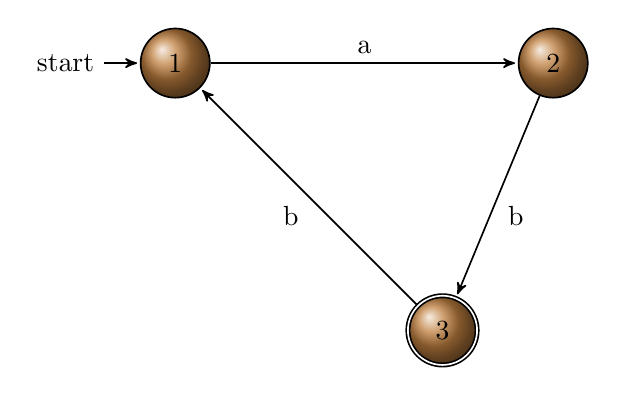
\begin{tikzpicture}[->,>=stealth',shorten >=1pt,auto,node distance=4.8cm, semithick]
\tikzstyle{every state}=[draw=black,text=black, ball color=brown]
\node[initial,state] (1) {1};
\node[state][right of=1](2){2};
\node[state, accepting][below right of=1](3){3};
\path (1)edge node{a}(2)
          (2)edge node{b}(3)
          (3)edge node{b}(1);       
\end{tikzpicture} 
\end{center}
\end{figure}
\section{}
\begin{enumerate}
\item Palindromes
\begin{proof}
For any regular language L, there exists a number p such that for any string w in L of length at least p there are strings x,y,z such that
\begin{enumerate}
\item If w = xyz.
\item And if x = a, y = b, z = a.
\item or if x = b, y = a, z = b.
\item Then $w = a^{90 + 1}ba^{90}$
\item and $w = b^{90 + 1}ab^{90}$
\item Therefore Palindromes are nonregular
\end{enumerate}
\end{proof}
\item Equal
\begin{proof}
For any regular language L, there exists a number p such that for any string w in L of length at least p there are strings x,y,z such that
\begin{enumerate}
\item  EQUAL = $\{\Lambda \quad ab \quad ba \quad aabb \quad abab \quad abba \quad baab \quad baba \quad bbaa \quad aaabbb...\}$
\item $\{a^nb^n\} = \mathbf{a^*b^*} \cap EQUAL$
\item If $a^*b^*$ is regular then so is the result of $\mathbf{a^*b^*} \cap EQUAL$
\item $w =  xyz$
\item $\mid xy \mid \le  p$
\item $\mid y \mid \ge 1$
\item Then $x = a^n, y = a^2, z = b^n$
\item So then xyyz would allow aaab which is not in this language.
\item Therefore this language is nonregular
\end{enumerate}
\end{proof}
\end{enumerate}
\section{}
Prove that the below generates the language defined by the regular expression: $\mathbf{a^*bb}$
$$\mathbf {Prod 1 \quad S \to aS \mid bb}$$
\begin{equation}
\begin{split}
&S \Longrightarrow aS\\
&\Longrightarrow aaS\\
&\Longrightarrow aaaS\\
&\Longrightarrow aaaaS\\
&\Longrightarrow aaaaaS\\
&\Longrightarrow aaaaabb\\
\end{split}
\end{equation}
This derivation could continue infinitely until terminal bb is appended.
\section{}
\begin{equation}
\begin{split}
&\mathbf {Prod 1 \quad S \to XaXaX}\\
&\mathbf {Prod 2 \quad X \to aX \mid bX \mid \Lambda}\\
\end{split}
\end{equation}
\section{}
\section{}
\end{document}